\message{ !name(rapport.tex)}

%% La classe stageM2R s'appuie sur la classe memoir, plus d'information sur le paquet: http://www.ctan.org/pkg/memoir
%% option possible de la classe stageM2R
% utf8  -> encodage du texte UTF8 (défaut: Latin1)
% final -> mode rapport de stage final (défaut: mode étude bibliographique)
% private -> indique une soutenance privée (défaut: soutenance publique)
\documentclass[utf8]{stageM2R} %-> etude bibliographique
%\documentclass[utf8,final]{stageM2R} %-> rapport final

\usepackage{wrapfig}
\usepackage{hhline}
\usepackage{subcaption}
\usepackage[]{algorithm2e}
\usepackage{amsthm}
\usepackage{mathtools}
\usepackage{float}
\usepackage{tikz}
\usepackage{tikz-qtree}
\usepackage{csquotes}
\usetikzlibrary{trees}
\usetikzlibrary{babel}
\usetikzlibrary{arrows,automata, positioning}

\usepackage[
    maxbibnames=9,
    maxnames=2,
    % style=nature,
    % citestyle=mla,
    backend=bibtex]
{biblatex}

\DeclareCiteCommand{\citeauthornsc}
  {\renewcommand*{\mkbibnamelast}[1]{####1}%
   \boolfalse{citetracker}%
   \boolfalse{pagetracker}%
   \usebibmacro{prenote}}
  {\ifciteindex
     {\indexnames{labelname}}
     {}%
   \printnames{labelname}}
  {\multicitedelim}
  {\usebibmacro{postnote}}

\DeclareCiteCommand*{\citeauthornsc}
  {\renewcommand*{\mkbibnamelast}[1]{####1}%
   \boolfalse{citetracker}%
   \boolfalse{pagetracker}%
   \usebibmacro{prenote}}
  {\ifciteindex
     {\indexnames{labelname}}
     {}%
   \printnames[][1-1]{labelname}}
  {\multicitedelim}
  {\usebibmacro{postnote}}



\bibliography{../../articles/biblio.bib}

% \newcommand*{\addheight}[2][.5ex]{%
%   \raisebox{0pt}[\dimexpr\height+(#1)\relax]{#2}%
% }

%%%%%%%%%%%%%%%%%%%%%%%%%%%%
%%% Déclaration du stage %%%
%%%%%%%%%%%%%%%%%%%%%%%%%%%%

%% auteur
\author{Noé Le Philippe}
%% encadrants
\supervisors{William Puech \\ Christophe Fiorio}
%% lieu du stage (Optionnel)
\location{Équipe ICAR - LIRMM UM5506 - CNRS, Université de Montpellier}
%% titre du stage
\title{La phylogénie des images dans les réseaux sociaux} 
%% parcours du master
\track{IMAGINA}  
%% date de soutenance (Optionnel)
\date{\today} 
%% version du rapport (Optionnel)
\version{1}
%% Résumé en francais
\abstractfr{
Ce stage de master.
}
%% Résumé en anglais
\abstracteng{
  This master thesis.
}



\begin{document}   

\message{ !name(rapport.tex) !offset(464) }
\ \frac{P_{i}}{Q_{i}}
\end{equation}
\\
La K divergence : 
\begin{equation}
  D_{kdiv}(P||Q) = \sum\limits_{i=1}^{d} P_{i}\ log\ \frac{2P_{i}}{P_{i}+Q_{i}}
\end{equation}


\chapter{Notre approche}
Ce chapitre sera consacré à présenter notre approche, nous y détaillerons notre approche, formalisée par un théorème, puis nous présenterons un algorithme permettant de reconstruire l'arbre de phylogénie.
\label{chap3}
\label{chap:notre_approche}
% \section{Principe}

% \fbox{
%   \parbox{\textwidth}{
%     \underline{Énoncé} :\\
%     Pour tout couple d'image (A, B), s'il n'est pas possible de prouver que A n'est pas le parent de B, alors il y a une relation parent-enfant entre A et B, A $\to$ B.
%   }
% }
% \\ \\ 
% \fbox{
%   \parbox{\textwidth}{
%     \underline{Preuve (empirique)} :\\
%     Si une fonction détecte à chaque fois qu'il est présent un marqueur prouvant qu'il n'y a pas de relation de parenté entre deux images, alors s'il n'en détecte pas c'est qu'il y a une relation de parenté entre les deux images.
%   }
% }

% \newtheorem*{parentage}{Théorème}
% \begin{parentage}
%   Pour tout couple d'images ($I_{m}$, $I_{n}$), s'il n'est pas possible de prouver que $I_{m}$ n'est pas le parent de $I_{n}$, alors il y a une relation parent-enfant entre $I_{m}$ et $I_{n}$, $I_{m}$ $\to$ $I_{n}$.
% \end{parentage}

% \begin{proof}
%   Soit $f(I_{m},I_{n})$ une fonction qui pour tout couple d'images $(I_{m}, I_{n})$ détecte à chaque fois qu'il est présent un marqueur prouvant qu'il n'y a pas de relation de parenté entre $I_{m}$ et $I_{n}$. Si $f(I_{m},I_{n})$ ne détecte rien alors c'est que $I_{m}$ est le parent de $I_{n}$.
% \end{proof}

\section{Principe et théorème}
Pour tout couple d'images de notre ensemble, nous allons tenter de nier qu'il existe une relation de parenté, cela va permettre d'extraire une matrice binaire, de la taille de l'ensemble d'image, où une case à vrai indiquera une relation de parenté. À noter une fois de plus que ce n'est pas forcément un parent direct mais plutôt un ancêtre. \\ \indent
Nous pouvons noter plusieurs choses intéressantes de l'exemple figure \ref{parentage_tree}. L'image $I_{2}$ a toute sa colonne marquée à vrai, c'est à dire que c'est un parent commun à toutes les autres images, et sa ligne n'a que des 0, elle n'a donc aucun parent. On se sert de ce principe pour la reconstruction de l'arbre à partir de la matrice : une image qui n'a pas de parent est donc la racine. Nous pouvons également remarquer les colonnes où toutes les cases sont à 0, cela veut dire que ces images ne sont les parents de personne, et donc sont des feuilles.

\begin{figure}
  \begin{subfigure}{.5\textwidth}
    \centering
    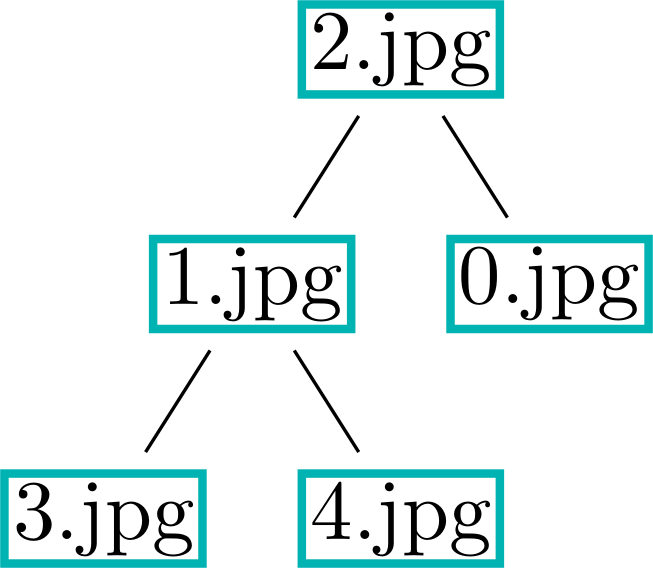
\includegraphics[width=.5\linewidth]{images/algo_tree.png}
    \caption{Arbre de phylogénie}
    \label{algo_tree}
  \end{subfigure}%
  \begin{subfigure}{.5\textwidth}
    \centering
    \begin{tabular}{|r||c|c|c|c|c|}
      \hline
      - & $I_{0}$ & $I_{1}$ & $I_{2}$ & $I_{3}$ & $I_{4}$ \\ \hhline{|=::=|=|=|=|=|}
      $I_{0}$ & - & 0 & 0 & 0 & 0 \\ \hline
      $I_{1}$ & 0 & - & 0 & 1 & 1 \\ \hline
      $I_{2}$ & 1 & 1 & - & 1 & 1 \\ \hline
      $I_{3}$ & 0 & 0 & 0 & - & 0 \\ \hline
      $I_{4}$ & 0 & 0 & 0 & 0 & - \\ \hline
    \end{tabular} 
    \caption{Matrice de parenté}
    \label{parentage_matrix}
  \end{subfigure}
  \caption{Une arbre de phylogénie et sa matrice de parenté.}
  \label{parentage_tree}
\end{figure}

Nous avons formalisé ce principe en un théorème : 
\newtheorem*{parentage}{Théorème}
\begin{parentage}
  Pour tout couple d'images ($I_{m}$, $I_{n}$), s'il n'est pas possible de prouver que $I_{m}$ n'est pas le parent de $I_{n}$, alors il y a une relation parent-enfant entre $I_{m}$ et $I_{n}$, $I_{m}$ $\to$ $I_{n}$.
\end{parentage}

\begin{proof}
  Soit $f(I_{m},I_{n})$ une fonction qui pour tout couple d'images $(I_{m}, I_{n})$ détecte à chaque fois qu'il est présent un marqueur prouvant qu'il n'y a pas de relation de parenté entre $I_{m}$ et $I_{n}$. Si $f(I_{m},I_{n})$ ne détecte rien alors c'est que $I_{m}$ est le parent de $I_{n}$, et donc $m < n$.
\end{proof}


\section{L'algorithme de reconstruction}
De ces quelques principes nous avons extrait un algorithme. \vspace{5mm}

\begin{algorithm}[H]
  % \SetAlgorithmName{MegaAlgorithm}{salut}
  \LinesNumbered
  \KwData{M a n$\times$n parentage matrix}
  \KwResult{the root of the tree}
  \BlankLine
  $nextRoot \leftarrow$ row with min sum of elements\;
  $treeRoot \leftarrow nextRoot$\;
  \BlankLine

  \ForAll{rows row of M}{
    $root \leftarrow nextRoot$\;
    mark $root$ as done\;
    \BlankLine
    \For{$i\leftarrow 0$ \KwTo n}{
      $row[i] \leftarrow 0$\;
      \If{sum of elements of row == 0} {
        add $i$ as child of $root$\;
      }
      \If{row has the smallest sum of elements and is not marked as done} {
        $nextRoot \leftarrow i$\;
      }
    }
  }
  \KwRet treeRoot
\caption{Construction de l'arbre}
\label{algo_}
\end{algorithm}
\vspace{5mm}

L'algorithme \ref{algo_} prend en entrée la matrice de parenté détaillée précédemment et retourne la racine de l'arbre. La philosophie de cet algorithme est qu'une image n'ayant aucun parent est la racine, et ce de manière récursive grâce à la structure d'arbre.

% La ligne 1 marque $nextRoot$ comme la ligne avec la plus petite somme des éléments, étant une matrice binaire, où les valeurs sont 0 et 1, c'est donc l'image qui a le moins de parent, autrement dit la racine.

% La ligne 5 marque $root$ comme terminée, c'est pour ne la traiter qu'une fois, en effet, dans un arbre, il n'y a pas de cycle, on ne peut donc pas 
% La condition lignes 8-10 ajoute l'image à l'indice $i$ comme enfant de $root$. La condition d'avoir tous les éléments de la ligne à 0, c'est à dire de n'avoir plus aucun parent

À chaque itération, une image est sélectionnée comme la racine (lignes 1 et 11) et nommée $root$, elle est retirée (ligne 7) des ancêtres des autres images si c'est un ancêtre. Si ces autres images n'ont plus d'ancêtre (ligne 8), c'est que $root$ était le parent direct de l'image en train d'être traitée, cette image est donc ajoutée comme enfant de $root$ (ligne 9). La ligne 5 permet de ne traiter qu'une fois chaque image comme racine potentielle.

Cet algorithme a une complexité de $O(n^{2})$. Il y a deux boucles imbriquées, et si les sommes sont calculées une une seule fois au début et mises à jour à chaque fois qu'un parent est enlevé, il n'y a pas de boucle supplémentaire augmentant la complexité.

Le but est donc de trouver la fonction permettant de détecter le marqueur prouvant qu'il n'y a pas de parenté. 
% Et même si cette fonction n'est pas parfaite, et qu'elle se trompe dans ses prédictions, l'algorithme est robuste et premet tout de même d'obtenir des résultats cohérents si on s'appuie sur les métriques introduites pas \autocite{dias2010first} pour évaluer l'arbre (voir Fig. \ref{algo-robuste}).

Il nous a semblé important, même dans le cadre de l'étude bibliographique, d'élaborer cet algorithme. Il est en effet assez simple mais néanmoins indispensable à notre méthode, et aurait pu orienter différemment nos recherche et notre méthode s'il n'avait pas été imaginé. Le reste du stage sera consacré à élaborer la fonction énoncée précédemment, en plus d'appliquer cet algorithme à plusieurs centaines d'exemples avec des configurations différentes pour pouvoir en tirer une analyse et une synthèse.

Cette approche a pour avantage de réduire l'évaluation d'un arbre de phylogénie à partir d'un ensemble d'images à l'évaluation binaire de parenté entre deux images.

%%%% faire une trace de l'algo %%%%%
\chapter{Conclusion}
\label{chap4}

% \nocite{*}
\printbibliography

\end{document}

\message{ !name(rapport.tex) !offset(-235) }
